\documentclass[14pt,a4paper]{scrartcl}
\usepackage{cmap}
\usepackage[utf8]{inputenc}
\usepackage[T1,T2A]{fontenc}
\usepackage[english,russian]{babel}
\usepackage{relsize}
\usepackage{graphicx}
\usepackage{subfigure}
\usepackage{mathtools}
\usepackage{amssymb}
\usepackage{float}
\usepackage{sidecap}
\usepackage{wrapfig}
\usepackage{caption}
\usepackage[table,xcdraw]{xcolor}
\usepackage{minted}
\begin{document}
	\begin{titlepage}
	\begin{center}
		\large
		МИНИСТЕРСТВО НАУКИ И ВЫСШЕГО ОБРАЗОВАНИЯ\\ РОССИЙСКОЙ ФЕДЕРАЦИИ
		
		\vspace{0.5cm}
		
		МГТУ им Н.Э.Баумана
		\vspace{0.25cm}
		
		Факультет ФН
		
		Кафедра вычислительной математики и математической физики
		\vfill
		
		
		Соколов Арсений Андреевич\\
		\vfill
		
		
		{\LARGE Домашнее задания №2 \\ по теории случайных процессов\\[2mm]
		}
		\bigskip
		
		3 курс, группа ФН11-63Б\\
		Вариант 19
	\end{center}
	\vfill
	
	\newlength{\ML}
	\settowidth{\ML}{«\underline{\hspace{0.7cm}}» \underline{\hspace{2cm}}}
	\hfill\begin{minipage}{0.4\textwidth}
		Преподаватель\\
		\underline{\hspace{3cm}} Т.\,В.~Облакова\\
		«\underline{\hspace{0.7cm}}» \underline{\hspace{1.71cm}} 2020 г.
	\end{minipage}%
	\bigskip
	
	
	\vfill
	
	\begin{center}
		Москва, 2020 г.
	\end{center}
\end{titlepage}

\section*{Задание 3}
Процесс изменения состояний системы $S$-однородный марковский процесс, заданный размеченным графом. Запишите систему уравнений Колмогорова для вероятностей состояний системы и найдите их предельные значения, если начальные условия имеют вид: $p_2 (0)=1$.\\
\textbf{Решение.}\\

Размеченный граф состояний системы $S$, процесс изменения состояния которой представляет собой однородный марковский процесс с дискретными состояниями изображён на рис. 1. 

%Составим систему дифференциальных уравнений Колмогорова, отталкиваясь от размеченного графа $S$-однородного марковского процесса, предоставленного по условию:

\begin{figure}[H]
	\begin{minipage}[h]{1\linewidth}
		\center{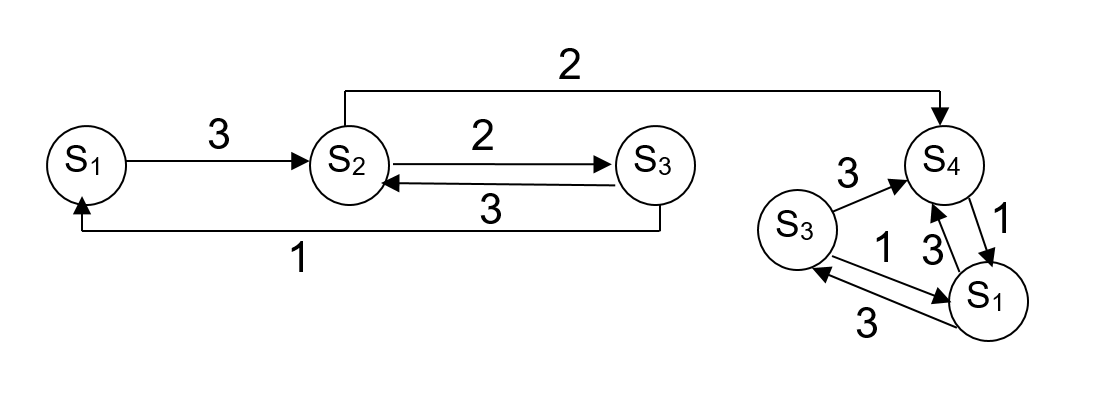
\includegraphics[width=1\linewidth]{../img/graph.png}}
		\caption{Размеченный граф состояний системы $S$\\}  
	\end{minipage}
\end{figure}



Сформулируем задачу Коши для системы уравнений Колмогорова (1), если $T = [0, \infty)$ и в начальный момент времени $t = 0$ система находится в состоянии (2)

\begin{equation}
	\begin{cases}
		p(t)' = \lambda(t)p(t), \quad t > 0;\\
		p(0) = p_0,
	\end{cases}
\end{equation}

где $\lambda(t) = \lambda$, так как рассматривается однородный марковский процесс, а сама матрица $\lambda$ вводится как указано далее. Пусть
\begin{equation*}
	I = (1 \; \ldots \; 1) \in M_{1n}(\mathbb{R});\\
\end{equation*} 
\begin{equation*}
	\lambda_k^0 = (\lambda_{k1} \; \ldots \; \lambda_{k,k-1} \; 0 \; \lambda_{k,k+1} \; \ldots \; \lambda_{kn})^T,
\end{equation*}
где $\lambda_{ki}$ для $i=\{\overline{1,n}\} \textbackslash \{k\}$ -- плотности вероятностей переходов системы $S$ из состояния $S_k$ во все иные возможные состояния, а
\begin{equation*}
	\lambda_{kk} = -I\lambda_k^0 = - \sum\limits_{\substack{i=1\\i\neq k}}^n \lambda_{ki} -
\end{equation*}
суммарная плотность вероятности перехода системы и состояния $s_k$ взятая со знаком "минус".


\begin{equation}
	p(0) = (0 \; 1 \; 0 \; 0 \; 0)^T
\end{equation}

Согласно заданному размеченному графу состояний, имеем

\begin{equation*}
\lambda(t) = \lambda = 
\begin{pmatrix}
-3 & 0 & 1 & 0 & 0 & 0\\
3 & -4 & 3 & 0 & 0 & 0 \\
0 & 2 & -4 & 0 & 0 & 0 \\
0 & 2 & 0 & -1 & 3 & 3 \\
0 & 0 & 0 & 0 & -4 & 3 \\
0 & 0 & 0 & 1 & 1 & -6 \\
\end{pmatrix}
\end{equation*}


Таким образом, вектор $p(t)$ вероятностей состояний изучаемой системы $S$ является решением следующей задачи Коши:

\begin{equation*}
	\begin{cases}
		p_1(t)' = -3p_1(t) + p_3(t);\\
		p_2(t)' = 3p_1(t) - 4p_2(t) + 3p_3(t);\\
		p_3(t)' = 2p_2(t) - 4p_3(t);\\
		p_4(t)' = 2p_2(t) - p_4(t) + 3p_5(t) + 3p_6(t);\\
		p_5(t)' = - 4p_5(t)+ 3p_6(t);\\
		p_6(t)' = p_4(t) + p_5(t) - 6p_6(t);\\
		
		p_2(0) = 1;\\
		p_k(0) = 0, \qquad k = \{1,3,4,5,6\}.
	\end{cases}
\end{equation*}


Перепишем систему в изображениях:

\begin{equation*}
	\begin{cases}
		s\widetilde{p_1}(s) - p_1(0) = -\widetilde{p_1}(s) + \widetilde{p_3}(s);\\
		s\widetilde{p_2}(s) - p_2(0) = 3\widetilde{p_1}(s) - 4\widetilde{p_2}(s) + 3\widetilde{p_3}(s);\\
		s\widetilde{p_3}(s) - p_3(0) = 2\widetilde{p_2}(s) - 4\widetilde{p_3}(s);\\
		s\widetilde{p_4}(s) - p_4(0) = 2\widetilde{p_2}(s) - 4\widetilde{p_4}(s) + 3\widetilde{p_5}(s) + 3\widetilde{p_6}(s);\\
		s\widetilde{p_5}(s) - p_5(0) = -4\widetilde{p_5}(s) + 3\widetilde{p_6}(s);\\
		s\widetilde{p_6}(s) - p_6(0) = \widetilde{p_4}(s) + \widetilde{p_5}(s) - 6\widetilde{p_6}(s);\\
		
		\widetilde{p_1}(s) + \widetilde{p_2}(s) + \widetilde{p_3}(s) + \widetilde{p_4}(s) + \widetilde{p_5}(s) + \widetilde{p_6}(s) = \frac{1}{s}.\\
	\end{cases}
\end{equation*}

Подставляя (2) получим:

\begin{equation*}
\begin{cases}
s\widetilde{p_1}(s) = -\widetilde{p_1}(s) + \widetilde{p_3}(s);\\
s\widetilde{p_2}(s) - 1 = 3\widetilde{p_1}(s) - 4\widetilde{p_2}(s) + 3\widetilde{p_3}(s);\\
s\widetilde{p_3}(s) = 2\widetilde{p_2}(s) - 4\widetilde{p_3}(s);\\
s\widetilde{p_4}(s) = 2\widetilde{p_2}(s) - 4\widetilde{p_4}(s) + 3\widetilde{p_5}(s) + 3\widetilde{p_6}(s);\\
s\widetilde{p_5}(s) = -4\widetilde{p_5}(s) + 3\widetilde{p_6}(s);\\
s\widetilde{p_6}(s) = \widetilde{p_4}(s) + \widetilde{p_5}(s) - 6\widetilde{p_6}(s);\\

\widetilde{p_1}(s) + \widetilde{p_2}(s) + \widetilde{p_3}(s) + \widetilde{p_4}(s) + \widetilde{p_5}(s) + \widetilde{p_6}(s) = \frac{1}{s}.\\
\end{cases}
\end{equation*}

Решая полученную систему, имеем:

\begin{equation*}
	\begin{cases}
		\widetilde{p_1}(s) = \frac{2}{s^{3}+9 s^{2}+18 s+4};\\
		\widetilde{p_2}(s) = \frac{s^{2}+5 s+4}{s^{3}+9 s^{2}+18 s+4};\\
		\widetilde{p_3}(s) = \frac{2(s+1)}{s^{3}+9 s^{2}+18 s+4};\\
		\widetilde{p_4}(s) = \frac{2(s+3)\left(s^{2}+5 s+2\right)}{(s+4) s\left(s^{3}+9 s^{2}+18 s+4\right)};\\
		\widetilde{p_5}(s) = \frac{6\left(s^{2}+5 s+2\right)}{s\left(s^{4}+16 s^{3}+81 s^{2}+130 s+28\right)(s+4)};\\
		\widetilde{p_6}(s) = \frac{2\left(s^{2}+5 s+2\right)}{s\left(s^{4}+16 s^{3}+81 s^{2}+130 s+28\right)};\\
	\end{cases}
\end{equation*}

Найдём предельные вероятности:

\begin{equation*}
	\Pi_k = \lim\limits_{t\rightarrow + \infty} p_k(t) = \lim\limits_{s\rightarrow 0 }s\widetilde{p_k}(s), \quad k=\overline{1,n}.
\end{equation*}

\begin{equation*}
	\begin{cases}
		\Pi_1 = 0;\\
		\Pi_2 = 0;\\
		\Pi_3 = 0;\\
		\Pi_4 = \frac{3}{4};\\
		\Pi_5 = \frac{3}{28};\\
		\Pi_6 = \frac{1}{7}.\\
	\end{cases}
\end{equation*}

Вектор финальных вероятностей:

\begin{equation*}
	\Pi = (0 \; 0 \; 0 \; \frac{3}{4} \; \frac{3}{28} \; \frac{1}{7}); \quad \frac{3}{4} + \frac{3}{28} + \frac{1}{7} = \frac{21}{28} + \frac{3}{28} + \frac{4}{28} = 1
\end{equation*}

%Заметим, что $\sum_{k=1}^{n=6} \Pi_k = 1$, что говорит о верности проделанных выше действий.\\
\textbf{Вывод.}\\
Полученный вектор финальных вероятностей соответствует очевидным соображениям о том, что изначальный граф состояний системы $S$, изображённый на рис. 1, состоит из двух подсистем: $S_A = {S_1, S_2, S_3}$ и $S_B = {S_4, S_5, S_6}$, причём при выходе из подсистемы $A$ обратно вернуться уже не получится. Поэтому значения $\Pi_1 , \Pi_2 , \Pi_3$ равны нулю.


\section*{Задание 4}
Требуется найти закон распределения времени пребывания марковского процесса в подмножестве состояний $U = \{S_2, S_3\}$, а также найти среднее время пребывания системы в $U$.\\

\textbf{Решение.}\\
Закон распределения времени пребывания Марковского процесса в подмножестве состояний $U = \{S_2,S_3\}$ имеет вид:
\begin{equation*}
	P_{T_{U}}(t)=\sum_{k=1}^{r}\left(\sum_{j=1}^{l} \lambda_{i_{k} j}\right) p_{i_{k}}(t)= 2p_2(t) + p_3(t)
\end{equation*}

Так как подмножество $U$ не замкнуто, найдём $p_2(t)$ и $p_3(t)$, решив систему:
\begin{equation*}
	\begin{cases}
		p_2(t)' = -4p_2(t) + 3p_3(t);\\
		p_3(t)' = -4p_3(t) + 2p_2(t).
	\end{cases}
\end{equation*}

Переходя к изображениями:

\begin{equation*}
	\begin{cases}
		s\widetilde{p_2}(s) - 1 = -4\widetilde{p_2}(s) + 3\widetilde{p_3}(s);\\
		s\widetilde{p_3}(s) = -4\widetilde{p_3}(s) + 2\widetilde{p_2}(s);\\
	\end{cases}
\end{equation*}

Получаем:

\begin{equation*}
	\begin{cases}
		\widetilde{p_2}(s) = \frac{s+4}{s^{2}+8 s+10};\\
		\widetilde{p_3}(s) = \frac{2}{s^{2}+8 s+10}
	\end{cases}
\end{equation*}


Возвращаясь к оригиналам:

\begin{equation*}
	\begin{cases}
		p_2(t) = {{\rm e}^{-4\,t}}\cosh \left( t\sqrt {6} \right) ; \\
		p_3(t) = 1/3\,\sqrt {6}{{\rm e}^{-4\,t}}\sinh \left( t\sqrt {6} \right) .
	\end{cases}
\end{equation*}

Тогда закон распределения времени пребывания Марковского процесса в подмножестве состояний $U = \{S_2,S_3\}$ имеет вид:

\begin{equation*}
	P_{T_{U}}(t) = 2p_2(t) + p_3(t) = \frac{\mathrm{e}^{-4 t}(\sqrt{6} \sinh (t \sqrt{6})+6 \cosh (t \sqrt{6}))}{3}
\end{equation*}


Найдём среднее время пребывания:

\begin{equation*}
	\begin{aligned}
		M \xi=\int\limits_{0}^{+\infty} x p_{\xi}(x) dx = \int\limits_{0}^{+\infty} \frac{\mathrm{e}^{-4 x}(\sqrt{3} \sinh (2 t \sqrt{3})+6 \cosh (2 x \sqrt{3}))}{3} dx = \frac{3}{5}
		\\
	\end{aligned}
\end{equation*}




\end{document}